\documentclass[oneside, DIV=11]{scrreprt}
\usepackage[utf8]{inputenc}
\usepackage{graphicx}

\usepackage{gensymb} % Pour le symbole degré

\usepackage[pdftex=true,hyperindex=true,linktocpage=true]{hyperref} % Pour les liens actifs dans le docs

% Pour les en-têtes et les pieds de page
\usepackage[]{fancyhdr}
\pagestyle{fancyplain}
\fancyhf{}
\fancyhead[L]{
\includegraphics[width=2cm]{img/text.png}}
\fancyhead[C]{Specifications}
\fancyhead[R]{\thepage/\pageref{LastPage}}

\fancyfoot[L]{The 2016 Hackaday Prize - Platform D}
\fancyfoot[R]{Alain Sanguinetti}
\renewcommand{\headrulewidth}{0pt}

\usepackage[english]{babel}

\title{Specifications of Platform D}
\author{}
\date{\today}

\begin{document}

\begin{titlepage}
    \begin{flushleft}
        {\sfb
            
\includegraphics[height=1cm]{img/text} \\[7cm]

            {\huge Platform D}\\[.5cm]
            {\LARGE Specifications }\\[.5cm]
            
            % A enlever :!!!!!!!!
            % ##########################################
            %{\large Version préliminaire }\\[2cm]
            % ##########################################
            
        }
        
        
        \vfill
        \emph{Alain Sanguinetti}\\
        \emph{The 2016 Hackaday Prize}
    \end{flushleft}
\end{titlepage}

\tableofcontents
\newpage

\chapter{Introduction}

\section{Project}


\section{Context}



\section{Challenge}

\chapter{Objectives and technical constraints}

\section{Functionnal analysis}
 (figure \ref{f1}).

\begin{figure}[h]
\centering
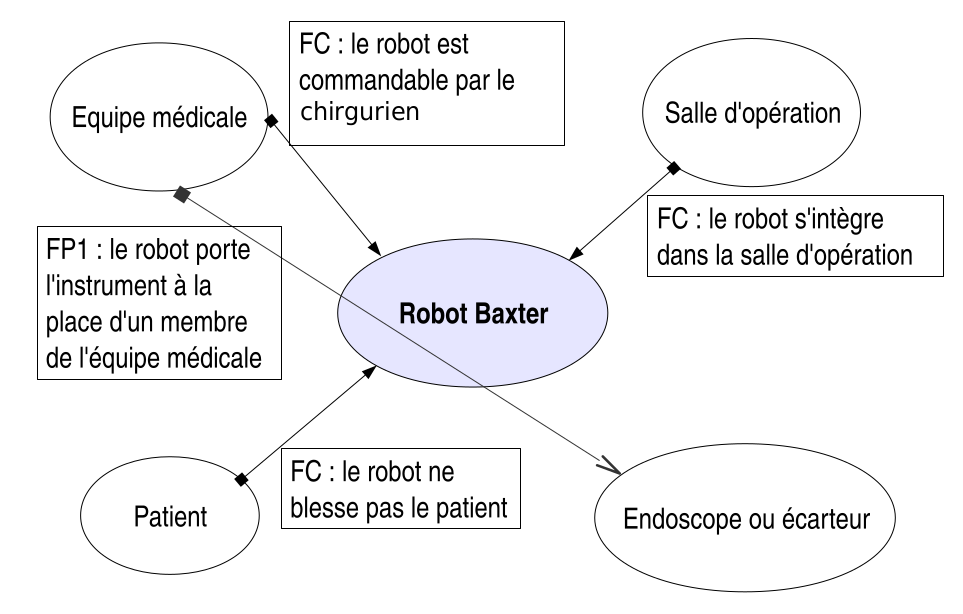
\includegraphics[width=0.85\textwidth]{img/grin2.png}
\caption{}
\label{f1}
\end{figure}



\section{}


\chapter{Project resources}

    \section{People}
    
    \section{Money}
    
    \section{Time}

    \section{Machines}

% La partie qui concerne le planning
\chapter{Calendar}

    \section{from April, 18th to April, 22nd}
    
    Specifications and Hackaday presentation is complete.
    If possible, document several technical solutions.
    
    \section{from April, 22nd to May, 30th}
    
    First build iteration. At least partially functionning prototype. 
    4 build logs on the Hackaday project page.

    \section{from May, 30th to July, 9th}
    
    Second build iteration.
    Document the kinematic equations and propose several designs for the legs that allow smooth movement and stability while not moving.
    Make some of the designs and test.
    Basic remote command.
    4 more build logs on the Hackaday project page.
    One video.
    
    \section{from July, 9th to July, 19th}
    
    Review and publish submission to the French Edition of the James Dyson Award.
    
    \section{from July, 19th to August, 22nd}
    
    Third build iteration.
    Stable and validated design, test mounting and powering of a robotized arm.
    Stable and robust command.

    \section{Optionnal, from August 22nd to Octover 3rd}

    I have no idea what my life is going to be like in this period.
    If possible, final release for hardware and software.

    \section{Outlook}
    
    This platform is only the beginning of my project. Next steps are integration of robotics arms and creating "macros" to automatize repetitive gardening tasks.

\chapter{Licensing}

\section{Project}


The project is released under the Peer Production License and Alain Sanguinetti is the sole owner of this project.

The license may be found on the follwing website: 

\url{http://p2pfoundation.net/Peer_Production_License}

\section{Third-party}
This project will use as much as possible free and open-source components in both hardware and software. 


% La page pour les signatures
\label{LastPage}

\end{document}
